\documentclass[journal]{IEEEtran}
\usepackage[a5paper, margin=10mm, onecolumn]{geometry}
\usepackage{tfrupee} % Include tfrupee package

\setlength{\headheight}{1cm} % Set the height of the header box
\setlength{\headsep}{0mm}     % Set the distance between the header box and the top of the text

\usepackage{gvv}
\usepackage{cite}
\usepackage{amsmath,amssymb,amsfonts,amsthm}
\usepackage{algorithmic}
\usepackage{graphicx}
\usepackage{textcomp}
\usepackage{xcolor}
\usepackage{txfonts}
\usepackage{listings}
\usepackage{enumitem}
\usepackage{mathtools}
\usepackage{gensymb}
\usepackage{comment}
\usepackage[breaklinks=true]{hyperref}
\usepackage{tkz-euclide} 
\usepackage{listings}
\def\inputGnumericTable{}                                 
\usepackage[latin1]{inputenc}                                
\usepackage{color}                                            
\usepackage{array}                                            
\usepackage{longtable}                                       
\usepackage{calc}                                             
\usepackage{multirow}                                         
\usepackage{hhline}                                           
\usepackage{ifthen}                                           
\usepackage{lscape}
\usepackage{float}
\begin{document}

\bibliographystyle{IEEEtran}
\vspace{3cm}


\renewcommand{\thefigure}{\theenumi}
\renewcommand{\thetable}{\theenumi}
\setlength{\intextsep}{10pt} % Space between text and floats

\numberwithin{equation}{enumi}
\numberwithin{figure}{enumi}
\renewcommand{\thetable}{\theenumi}

% --- End of page settings ---

\pagenumbering{roman} 
\begin{titlepage}
\begin{center}
\vfill
\vspace{6cm}
\hrule
\vspace{.5cm}
{\huge \bfseries SCIENTIFIC CALCULATOR} % title of the report
\vspace{.5cm}

\hrule
\vspace{1.5cm}

\textsc{\textbf{By}}\\
\vspace{.5cm}

% add your name here
K. AKHIL - EE24BTECH11035\\

\vspace{2cm}

\today % see latexmkrc for time zone change

\vfill
\end{center}
\end{titlepage}


\newpage

%\addcontentsline{toc}{section}{Table of Contents}
\renewcommand{\baselinestretch}{1}\normalsize
\tableofcontents
\renewcommand{\baselinestretch}{1}\normalsize
%\singlespacing
\thispagestyle{fancy} % force page style

\newpage
\pagenumbering{arabic} 

\section{Required Components} \label{ch1}
\input{sources/Required Components.tex} 
\label{EndOfText}


\pagenumbering{arabic} 

\section{Hardware Connections} \label{ch1}
\begin{table}[h]
    \centering
    \renewcommand{\arraystretch}{1.3}  % Adjust row height
    \begin{tabular}{|c|c|c|}
        \hline
        \textbf{Component} & \textbf{ATmega328P Pin} & \textbf{Connection Description} \\
        \hline
        BCD Input A & Digital Pin 2 & Connected to 7447 A input \\
        BCD Input B & Digital Pin 3 & Connected to 7447 B input \\
        BCD Input C & Digital Pin 4 & Connected to 7447 C input \\
        BCD Input D & Digital Pin 5 & Connected to 7447 D input \\
        \hline
        COM (Tens Place) & Analog Pin A3 (PC3) & Common pin for 7-segment (Tens) \\
        COM (Units Place) & Analog Pin A4 (PC4) & Common pin for 7-segment (Units) \\
        \hline
        7-Segment Display & 7447 Output & 7447 drives segments \\
        \hline
    \end{tabular}
    \vspace{0.5cm}
    \caption{Pin Connections for 7-Segment Display with 7447 and ATmega328P}
\end{table}
\begin{figure}[H]
    \centering
    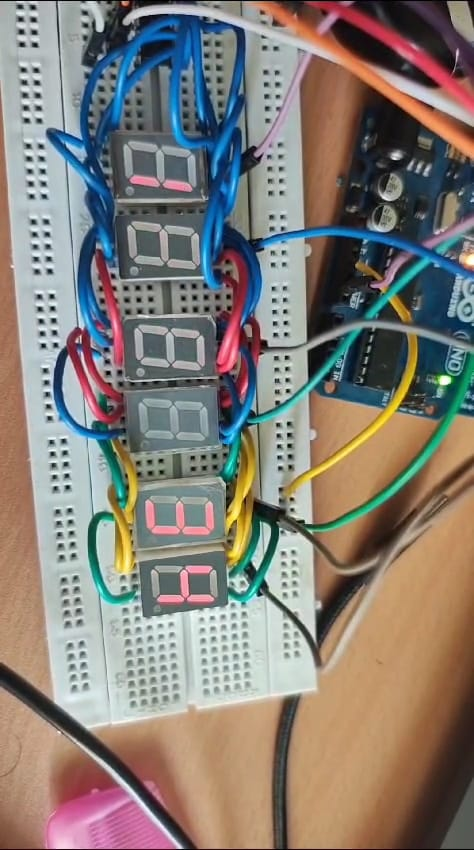
\includegraphics[width=0.35\linewidth]{WhatsApp Image 2025-03-24 at 18.30.23_1f184068.jpg}
    \caption{}
    \label{fig:enter-label}
\end{figure} 
\label{EndOfText}
\pagenumbering{arabic} 

\section{Working Explanation } \label{ch1}


\subsection{Initialization of I/O and Timer}
The ATmega328P microcontroller initializes the required I/O pins and configures Timer1 for interrupt-driven time updates.

\begin{itemize}
    \item The BCD pins (A, B, C, D) are configured as outputs to send data to the 7447 decoder.
    \item The common anodes of the six seven-segment displays are connected to separate Arduino analog pins.
    \item Timer1 is configured to trigger an interrupt every 1 second to increment time.
\end{itemize}

\subsection{Displaying Time Using Multiplexing}
The clock utilizes multiplexing to drive six seven-segment displays efficiently while minimizing the number of required I/O pins.

\begin{enumerate}
    \item The digits for hours, minutes, and seconds are extracted from the stored time values using bitwise operations.
    \item The appropriate BCD values are sent to the 7447 decoder.
    \item Only one display is activated at a time using the corresponding common anode pin.
    \item A short delay ensures proper visibility before switching to the next digit.
    \item This rapid switching occurs continuously, giving the illusion that all digits are displayed simultaneously.
\end{enumerate}

\subsection{Time Keeping and Increment Logic}
The microcontroller stores time values in BCD format, ensuring efficient calculations and display updates.

\begin{itemize}
    \item The seconds value increments every time the Timer1 interrupt triggers.
    \item If seconds reach 60, they reset to 00, and the minutes value increments.
    \item If minutes reach 60, they reset to 00, and the hours value increments.
    \item If hours reach 24, they reset to 00, completing a full-day cycle.
\end{itemize}

\subsection{Timer1 Interrupt for Precise Timing}
Timer1 is configured in **Clear Timer on Compare Match (CTC) Mode** to generate precise 1-second interrupts.

\begin{enumerate}
    \item The Timer1 interrupt is triggered every second using a compare match value calculated for a 16MHz clock.
    \item When the interrupt occurs, the seconds counter increments.
    \item If a carry-over condition is met, minutes and hours are updated accordingly.
    \item The updated time values are sent to the display in the next iteration.
\end{enumerate}

\subsection{Main Loop Execution}
The `main()` function continuously updates the display while the Timer1 interrupt manages time increments in the background.

\begin{itemize}
    \item The main loop does not block execution with delays, ensuring smooth operation.
    \item Display updates occur independently of the timekeeping logic, preventing flickering or lag.
    \item The system can be expanded to include additional functionality, such as setting the time using push buttons.
\end{itemize}
 
\label{EndOfText}
\label{endOfDoc}

\pagenumbering{arabic} 

\section{Code Outline $&$ Explanation } \label{ch1}

\definecolor{codebg}{rgb}{0.95,0.95,0.95}
\lstset{
    backgroundcolor=\color{codebg},
    basicstyle=\ttfamily\footnotesize,
    keywordstyle=\color{blue}\bfseries,
    commentstyle=\color{green!50!black},
    numbers=left,
    numberstyle=\tiny\color{gray},
    frame=single,
    breaklines=true
}
\subsection*{Defining CPU Frequency}
\begin{lstlisting}
#define F_CPU 16000000UL
\end{lstlisting}
The microcontroller runs at 16 MHz. This definition ensures proper timing calculations.

\subsection*{Including Required Headers}
\begin{lstlisting}
#include <avr/io.h>
#include <avr/interrupt.h>
#include <util/delay.h>
\end{lstlisting}
These headers provide functions for I/O operations, interrupt handling, and delays.

\subsection*{Defining BCD and Display Control Pins}
\begin{lstlisting}
#define A PD2  
#define B PD3  
#define C PD4  
#define D PD5  

#define H1 PD6  
#define H2 PD7  
#define M1 PB0  
#define M2 PB1  
#define S1 PB2  
#define S2 PB3  
\end{lstlisting}
- **PD2–PD5** are connected to the 7447 BCD decoder.
- **PD6, PD7, PB0–PB3** control which digit is active.

\subsection*{Clock Variables in BCD Format}
\begin{lstlisting}
volatile uint8_t hours = 0b00010010;
volatile uint8_t minutes = 0b00000000;
volatile uint8_t seconds = 0b00000000;
\end{lstlisting}
The time is stored in **Binary-Coded Decimal (BCD)** format.

\subsection*{Displaying a Single Digit}
\begin{lstlisting}
void displayDigit(uint8_t digit) {
    PORTD = (PORTD & 0b11000011) | (digit << 0b00000010);
}
\end{lstlisting}
This function sends a **BCD digit** to **PORTD (PD2–PD5)** while preserving other bits.

\subsection*{Displaying the Complete Time}
\begin{lstlisting}
void displayTime() {
    uint8_t h1 = (hours >> 4) & 0x0F;
    uint8_t h2 = hours & 0x0F;
    uint8_t m1 = (minutes >> 4) & 0x0F;
    uint8_t m2 = minutes & 0x0F;
    uint8_t s1 = (seconds >> 4) & 0x0F;
    uint8_t s2 = seconds & 0x0F;

    PORTD |= (1 << H1); displayDigit(h1); _delay_ms(5); PORTD &= ~(1 << H1);
    PORTD |= (1 << H2); displayDigit(h2); _delay_ms(5); PORTD &= ~(1 << H2);
    PORTB |= (1 << M1); displayDigit(m1); _delay_ms(5); PORTB &= ~(1 << M1);
    PORTB |= (1 << M2); displayDigit(m2); _delay_ms(5); PORTB &= ~(1 << M2);
    PORTB |= (1 << S1); displayDigit(s1); _delay_ms(5); PORTB &= ~(1 << S1);
    PORTB |= (1 << S2); displayDigit(s2); _delay_ms(5); PORTB &= ~(1 << S2);
}
\end{lstlisting}
- Extracts each **tens** and **units** place digit using bitwise operations.
- Uses **multiplexing** to display each digit sequentially.

\subsection*{Timer Interrupt for 1-Second Updates}
\begin{lstlisting}
ISR(TIMER1_COMPA_vect) {
    seconds += 1;
    if ((seconds & 0x0F) > 9) { 
        seconds = (seconds & 0xF0) + 0x10;
    }
    if (seconds >= 0x60) {
        seconds = 0x00;
        minutes += 1;
    }
    if ((minutes & 0x0F) > 9) { 
        minutes = (minutes & 0xF0) + 0x10;
    }
    if (minutes >= 0x60) {
        minutes = 0x00;
        hours += 1;
    }
    if ((hours & 0x0F) > 9) { 
        hours = (hours & 0xF0) + 0x10;
    }
    if (hours >= 0x24) {
        hours = 0x00;
    }
}
\end{lstlisting}
- Increments **seconds** every timer interrupt (1 second).
- **Handles carry propagation** from seconds → minutes → hours.

\subsection*{Timer1 Configuration}
\begin{lstlisting}
void timer1_init() {
    TCCR1B |= (1 << WGM12) | (1 << CS12) | (1 << CS10);
    OCR1A = 15624;
    TIMSK1 |= (1 << OCIE1A);
    sei();
}
\end{lstlisting}
- **Sets Timer1 to CTC mode**.
- **Prescaler 1024** → Results in **1-second intervals**.
- Enables **interrupts** on compare match.

\subsection*{Main Function}
\begin{lstlisting}
int main(void) {
    DDRD |= (1 << A) | (1 << B) | (1 << C) | (1 << D);
    DDRD |= (1 << H1) | (1 << H2);
    DDRB |= (1 << M1) | (1 << M2) | (1 << S1) | (1 << S2);
    
    timer1_init();

    while (1) {
        displayTime();
    }
}
\end{lstlisting}
- **Configures I/O pins** for **BCD outputs** and **digit control**.
- **Starts Timer1** for automatic timekeeping.
- **Continuously updates the display** in an infinite loop.
 
\label{EndOfText}
\label{endOfDoc}
\newpage
\pagenumbering{arabic} 

\section{Conclusion} \label{ch1}
This project successfully implements a digital clock using an ATmega328P microcontroller, seven-segment displays, and a 7447 BCD to 7-segment decoder. The clock accurately displays time in the HH:MM:SS format by utilizing a hardware timer interrupt for precise timekeeping.

Key takeaways from this project include:
\begin{itemize}
    \item Efficient multiplexing: Controlling multiple 7-segment displays using limited I/O pins.
    \item Precise timing: Achieved using Timer1 interrupt to increment seconds every second.
    \item BCD-based storage: Ensuring correct representation of time without complex conversions.
    \item Modularity and expandability: The system can be modified for real-time clock (RTC) modules or additional features like alarms.
\end{itemize}

This project demonstrates how microcontrollers can be used for real-time applications, providing a foundation for more advanced embedded systems. Future improvements may include RTC integration, battery backup, or OLED/LCD display support for enhanced functionality. 
\label{EndOfText}
\label{endOfDoc}
\newpage
\pagenumbering{arabic} 

\section{References} \label{ch1}
\input{sources/references} 
\label{EndOfText}
\label{endOfDoc}
\end{document}
